\section{Ziel}
\label{sec:Ziel}
Der \textsc{Frank}--\textsc{Hertz}-Versuch zählt zu den Elektronenstoßexperimenten. 
Diese werden genutzt, um die Struktur der Elektronenhülle eines Atoms genauer zu erforschen.
Ziel ist es, die Anregungsenergie eines Quecksilberatomes zu bestimmen, die Energieverteilung der stoßenden Elektronen zu untersuchen, sowie die Ionisierungsenergie von Quecksilber zu beziffern.

\section{Theorie}
\label{sec:Theorie}
\subsection{Anregung eines Hg-Atoms}
Zur Bestimmung der Anregungsenergie eines Quecksilberatoms wird dieses mit Elektronen bestimmter Energie beschossen.
Die Elektronen übertragen durch Stoßprozesse ihre Energie auf das Atom und versetzen es in einen angeregten Zustand.
Aus den Informationen des Energieverlustes der stoßenden Elektronen können Rückschlüsse auf die Anregungsenergie $E_\mathup{a}$ gezogen werden. 
Stoßen Hg-Atom und Elektron unelastisch, so nimmt das Atom die Energie
\begin{equation}
	\label{eq:E_a}
	\frac{m_\mathup{e} v_\mathup{vor}²}{2}-\frac{m_\mathup{e} 	v_\mathup{nach}²}{2}=E_1-E_0=E_\mathup{a}
\end{equation}
auf.
$m_\mathup{e}$ bezeichnet die Masse der stoßenden Elektronen, $v_i$ ihre Geschwindigkeit vor und nach dem Stoß, $E_0$ die Energie des Hg-Atoms im Grund- und $E_1$ die Energie im ersten angeregten Zustand. 
Nach einer Relaxationszeit von $t \approx \SI{1e-8}{\second}$ geht das Hg-Atom wieder in den Grundzustand über. Dabei wird ein Lichtquant der Energie
\begin{equation}
	h \nu =E_1-E_0
\end{equation}
emittiert.
Ein unelastischer Stoß kommt zustande, wenn für die Energie der stoßenenden Elektronen die Bedingung $E_\mathup{e} \geq E_\mathup{a}$ gilt. 
Wird diese nicht erfüllt stoßen Elektron und Atom elastisch. 
Es kommt aufgrund des großen Massenunterschiedes zu einer geringen Energieabgabe.
%von 
%\begin{equation}
%	\Delta E=\frac{4m_\mathup{e}M}{(m_\mathup{e}+M)²}\cdot 		E_	\mathup{e} \approx 1,1\cdot 10⁻⁵ E_\mathup{e}
%\end{equation}
Es kommt zur Richtungsänderung der Elektronen.
%Dieser kleine Energiebetrag ruft eine Richtungsänderung des Elektrons hervor, führt jedoch nicht zu einer Anregung der Atome.

\subsection{Idealisierte \textsc{Franck}-\textsc{Hertz}-Kurve}
\begin{figure}
	\centering
	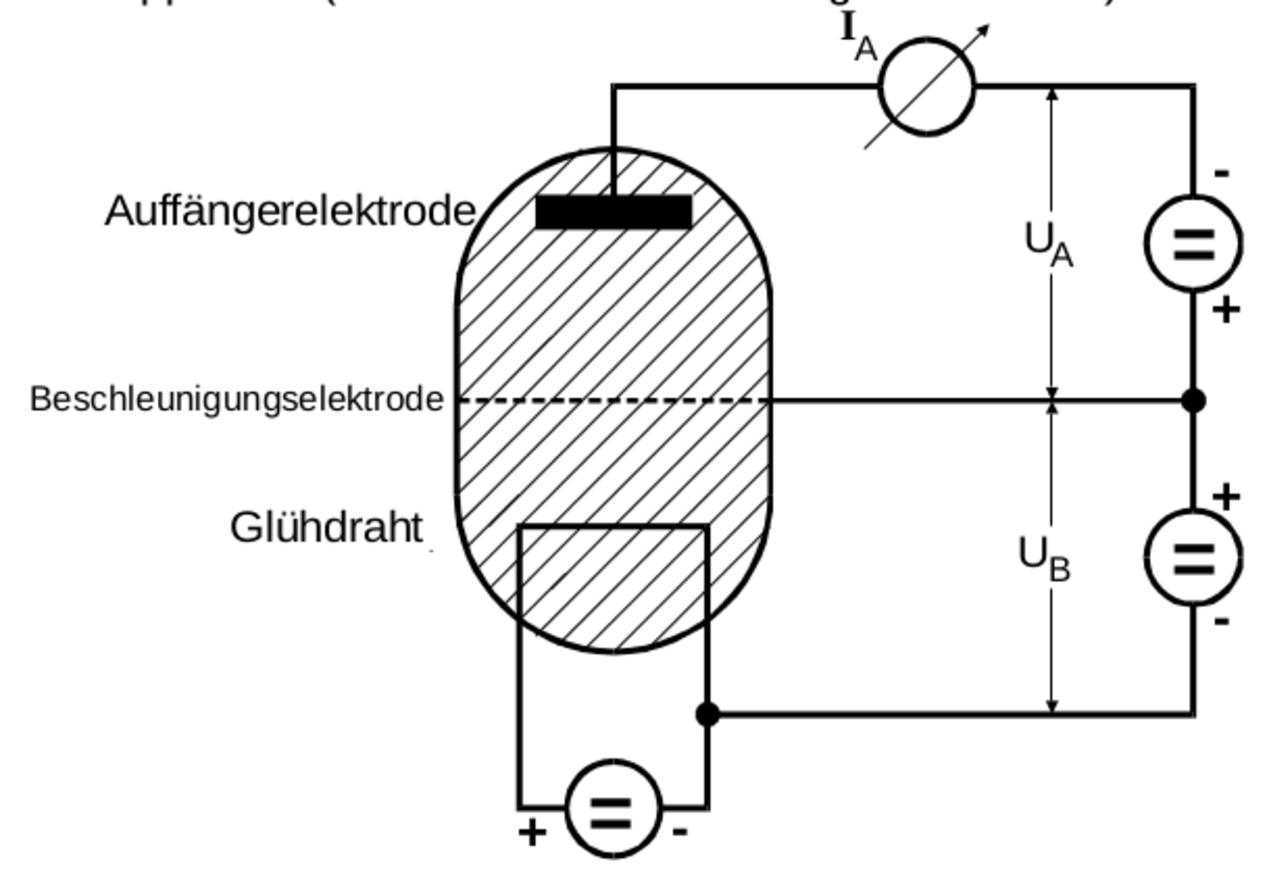
\includegraphics[width=0.6\textwidth]{Bilder/Aufbau.pdf}
	\caption{Aufbau der \textsc{Franck}--\textsc{Hertz}-Kurve.\cite{skript}}
\end{figure}
In einem evakuierten Glasgefäß befindet sich ein Tropfen Quecksilber (Hg), der teilweise verdampft. 
Abhängig von der Umgebungstemperatur $T$ bildet sich ein Gleichgewichtsdampfdruck $p_\mathup{sät}$ aus. 
Ein heißer Glühdraht dient als Elektronenlieferant.
Durch eine gitterförmige Beschleunigungselektrode mit positiver Beschleunigungsspannung $U_\mathup{B}$ wird den Elektronen eine Energie von 
\begin{equation}
	e U_\mathup{B}=\frac{m_\mathup{e}v_\mathup{vor}²}{2}
\end{equation}
zugeführt. 
Erreichen die Elektronen die Auffängerelektrode lässt sich ein Auffängerstrom $I_\mathup{A}$ messen. 
Elektronen treffen jedoch nur auf die Auffängerelektrode, wenn sie genug Energie besitzen um zuvor deren Bremsfeld, erzeugt durch die Spannung $U_\mathup{A}$, zu überwinden. 
Nur Elektronen mit 
\begin{equation}
	\frac{m_\mathup{e}}{2}v_\mathup{z}² \geq e U_\mathup{A}
\end{equation}
passieren diese Hürde -- die restlichen Elektronen kehren zur Beschleunigerelektrode zurück.
Zur Bestimmung der Anregungsenergie wird die zuvor erwähnte Gegenfeldmethode benutzt. 
Während die Elektronen sich durch das Gefäß bewegen stoßen sie mit den Hg-Atomen zusammen. 
Das Beobachten des Auffängerstroms $I_\mathup{A}$ gibt Aufschluss über die Anregungsenergie.
Ein Erhöhen von $U_\mathup{B}$ lässt den Strom ansteigen, da immer mehr Elektronen die Auffängerelektrode erreichen.
Sobald die Elektronen eine Energie aufweisen, die gleich der Anregungsenergie von Quecksilber ist, geben sie diese durch Stöße an die Hg-Atome ab. 
Danach reicht ihre Energie nicht mehr aus, um das Gegenfeld zu passieren -- $I_\mathup{A}$ fällt rasant ab.
Starkes Erhöhen von $U_\mathup{B}$ führt den Elektronen so viel Energie zu, dass mehrere Stöße ermöglicht werden. 
Die Abstände der Maxima $U_1$ in Abbildung \ref{fig:id} entsprechen der Anregungsenergie des Hg-Atoms im ersten Zustand:
\begin{equation}
	U_1=\frac{1}{e_0}{(E_1-E_0)}.
\end{equation}
\begin{figure}
	\centering
	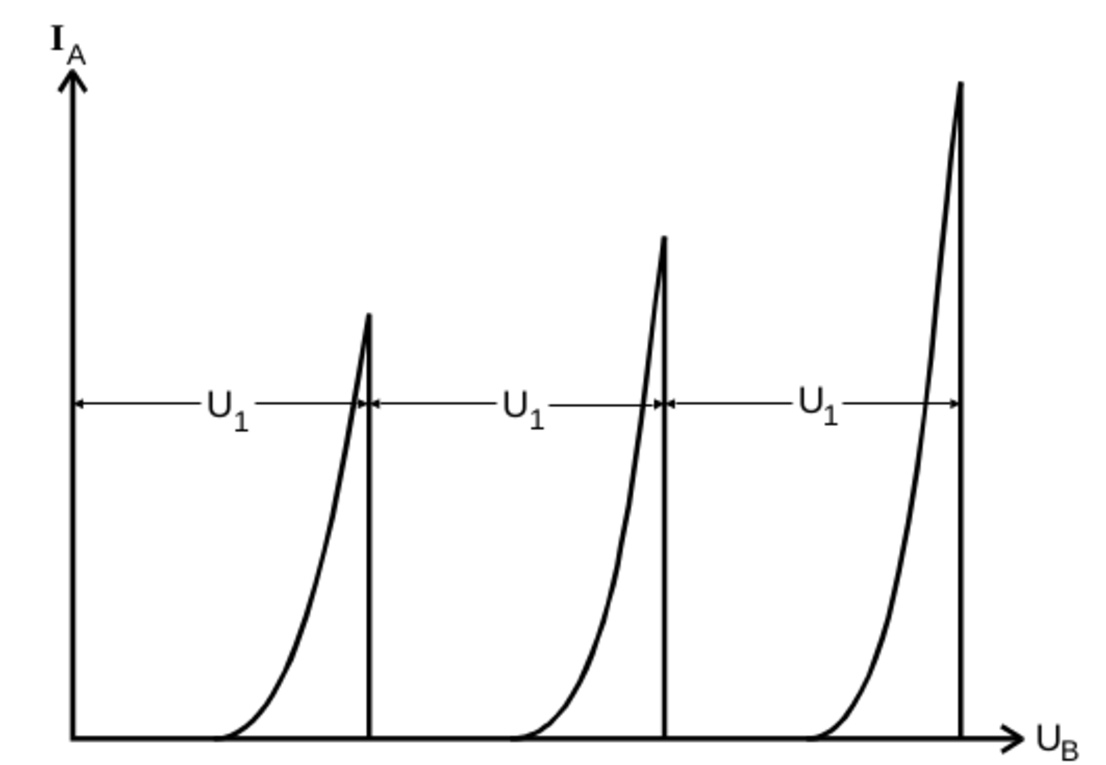
\includegraphics[width=0.5\textwidth]{Bilder/Kurve_Theo.pdf}
	\caption{Idealisierter Kurvenverlauf des Auffängerstroms $I_\mathup{A}$.\cite{skript}}
	\label{fig:id}
\end{figure}
Der tatsächliche Kurvenverlauf weicht vom idealen etwas ab, da einige messbedingte Nebeneffekte auftreten.

\subsubsection{Nebeneffekte}
\begin{enumerate}
\item{Das Kontaktpotential}

Die eingestellte Spannung $U_\mathup{B}$ unterscheidet sich von der tatsächlichen Beschleunigungsspannung. 
Grund dafür sind die Potentiale $\phi_\mathup{D}$ und $\phi_\mathup{BE}$ , d.h. die Austrittsarbeit der Elektronen aus verwendetem Glühdraht und der Beschleunigerelektrode. 
Diese unterscheiden sich dank unterschiedlichem Material.
Die Effektivspannung ist um den Betrag des Kontaktpotentials $k$ herabgesetzt und die Kurve deswegen um $k$ mit
\begin{equation}
	U_\mathup{B,eff}=U_\mathup{B}-\frac{1}{\epsilon_0}(\phi_\mathup{BE}-\phi_\mathup{D})=U_\mathup{B}-k
\end{equation}
verschoben.
\item{Energiespektrum der Elektronen}

Nach der \textsc{Fermi}--\textsc{Dirac}-Verteilung weisen die Leitungselektronen eines Metalls ein Energiespektrum auf und besitzen damit unterschiedliche Anfangsgeschwindigkeiten, sobald sie aus dem Glühdraht austreten.
Das hat zur Folge, dass die Kurvenmaxima sich langsamer ausbilden und flacher werden. 
Außerdem ist kein unstetiger Abfall der Kurve auf ein Stromminimum von $I_\mathup{A}=0\,\si\volt$ zu beobachten.
Richtungsänderungen eventueller elastischer Stöße führen zu einer Verbreiterung des Kurvenverlaufs, sofern diese zwischen Beschleuniger- und Auffängerelektrode stattfinden. 
\item{Dampfdruck}

Für die mittlere freie Weglänge $\overline{w}$ muss $\overline{w} << a$ mit dem Abstand $a$ zwischen beiden Elektroden gelten, um die Wahrscheinlichkeit unelastischer Stöße zu maximieren. 
$\overline{w}$ ist über den Dampfdruck $p_\mathup{sät}$ steuerbar. Dieser wird über die Temperatur $T$ eingestellt. 
\begin{align}
	\overline{w}=\frac{0,0029}{p_\mathup{sät}}\qquad\\
	p_\mathup{sät}(T)=5,5\cdot 10⁷\exp{-\frac{6876}{T}}, [p_\mathup{sät}]=\si{\milli\bar}, [\overline{w}]=\si{\centi\meter}.
\end{align}
In einem bestimmten Temperaturbereich ist die Stoßwahrscheinlichkeit optimal.
Ein kleinerer Druck bei geringer Temperatur führt zu einer geringen Stoßwahrscheinlichkeit, ein größerer Druck bei hoher Temperatur führt zu vielen elastischen Stößen.
\end{enumerate}
